\documentclass{standalone}

\usepackage{tikz}

\begin{document}

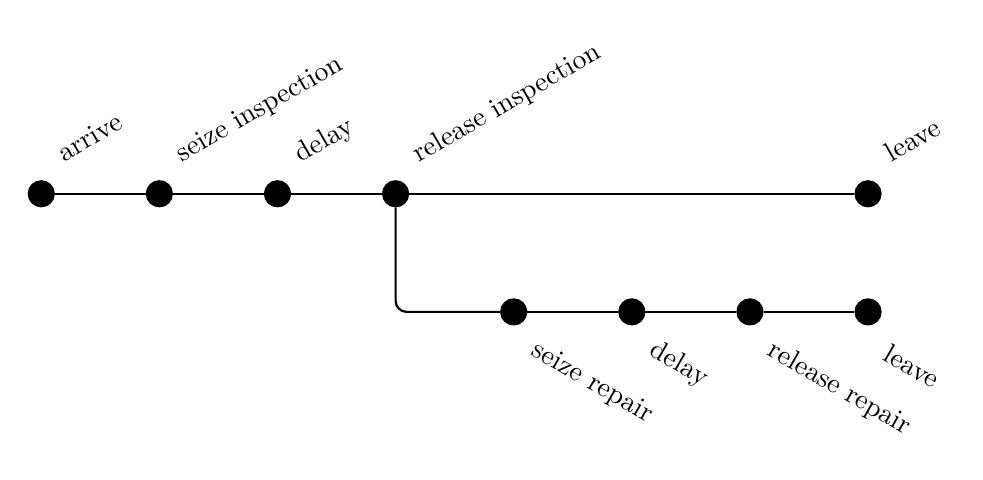
\begin{tikzpicture}
  
\node[circle, draw=black, fill=black] (arrive) at (0, 0) {};
\node[rotate=30, anchor=north west] at (0, 0.65) {arrive};
\node[circle, draw=black, fill=black] (inspection_seize) at (1.5, 0) {};
\node[rotate=30, anchor=north west] at (1.5, 0.65) {seize inspection};
\node[circle, draw=black, fill=black] (inspection_delay) at (3, 0) {};
\node[rotate=30, anchor=north west] at (3., 0.65) {delay};
\node[circle, draw=black, fill=black] (inspection_release) at (4.5, 0) {};
\node[rotate=30, anchor=north west] at (4.5, 0.65) {release inspection};
\node[circle, draw=black, fill=black] (inspection_leave) at (10.5, 0) {};
\node[rotate=30, anchor=north west] at (10.5, 0.65) {leave};
\node[circle, draw=black, fill=black] (repair_seize) at (6, -1.5) {};
\node[rotate=-30, anchor=south west] at (6., -2.15) {seize repair};
\node[circle, draw=black, fill=black] (repair_delay) at (7.5, -1.5) {};
\node[rotate=-30, anchor=south west] at (7.5, -2.15) {delay};
\node[circle, draw=black, fill=black] (repair_release) at (9, -1.5) {};
\node[rotate=-30, anchor=south west] at (9., -2.15) {release repair};
\node[circle, draw=black, fill=black] (repair_leave) at (10.5, -1.5) {};
\node[rotate=-30, anchor=south west] at (10.5, -2.15) {leave};

\draw[thick] (arrive) -- (inspection_seize);
\draw[thick] (inspection_seize) -- (inspection_delay);
\draw[thick] (inspection_delay) -- (inspection_release);
\draw[thick] (inspection_release) -- (inspection_leave);
\draw[thick, rounded corners] (inspection_release) -- (4.5, -1.5) -- (repair_seize);
\draw[thick] (repair_seize) -- (repair_delay);
\draw[thick] (repair_delay) -- (repair_release);
\draw[thick] (repair_release) -- (repair_leave);

\end{tikzpicture}

\end{document}
